\subsubsection{\stid{5.01} Software Development Kits} \label{subsubsect:ecosystem-sdk}

\paragraph{Overview} The ST Software Development Kit (SDK) project supports a set of activities aimed at

\begin{itemize}
\item establishing Community Policies aimed at increasing the interoperability between and sustainability of ST software packages, using the xSDK~\cite{xsdk:homepage} community package and installation policies~\cite{xsdk-policies:homepage} as a model.

\item coordinating the delivery of ECP ST products through the Extreme-Scale Scientific Software Stack (E4S)~\cite{e4s:homepage}, a comprehensive and coherent set of software tools, to all interested stakeholders on behalf of ECP ST. This includes ECP applications and the broader open source community.
\end{itemize}

An ECP ST SDK is a collection of related software products (called packages) where coordination across package teams will improve usability and practices and foster community growth among teams that develop similar and complementary capabilities.  SDKs have the following attributes:
\begin{itemize}
\item Domain scope: Collection makes functional sense.
\item Interaction model: How packages interact; compatible, complementary, interoperable.
\item Community policies: Value statements; serve as criteria for membership.
\item Community interaction: Communication between teams. Bridge culture. Common vocabulary.
\item Meta-infrastructure: Encapsulates, invokes build of all packages (Spack), shared test suites.
\item Coordinated plans: Inter-package planning. Does not replace autonomous package planning.
\item Community outreach: Coordinated, combined tutorials, documentation, best practices.
\end{itemize}

The SDK project is needed within ECP because it will make it simpler for ECP applications to access required software dependencies on ECP target platforms and drastically lower the cost of exploring the use of additional ECP ST software that may be of benefit. In addition, the SDK effort will decrease the ECP software support burden at the major computing facilities by ensuring the general compatibility of ST packages within a single software environment, providing tool support for the installation of ST packages on facility machines, communicating common requirements for ST software and facilitating the set up of CI testing on facility platforms. This project will work closely with the HI 2.4.4 \textit{Deployment of Software at the Facilities} project.

\paragraph{Key  Challenges}
ST software packages have been developed in a variety of very different cultures and are at significantly different levels of software engineering maturity and sophistication. The experience of some of the SDK staff during the formation of the xSDK showed that in this situation, it is challenging to establish common terminology and effective communication, and these are prerequisites to community policies and a robust software release.

Deciding exactly how to deploy the SDKs at the facilities is itself a challenge. ECP applications will use different combinations of ST software in different configurations. For example, applications will want mathematical libraries capabilities from the xSDK build on top of both MPICH and OpenMPI, and will want different configurations of those mathematical libraries.

\paragraph{Solution Strategy}
The SDK solution strategy involves pursuing interoperability and sustainability goals by grouping ST software projects into logical collections whose members will benefit from a common set of community policies as well as increased communication between members to standardize approaches where sensible and establish better software practices. 

The SDK effort will also facilitate the use of common infrastructure, such as CI testing at the major computing facilities and the Spack~\cite{gamblin+:sc15} package manager. SDK release and delivery goals will benefit from common package manager and testing infrastructure. In addition to the delivery of the E4S through Spack, the SDK will also explore the option of binary delivery, possibly through OpenHPC.

Recognizing the different release readiness and broader maturity differences between different ECP ST products, the early release strategy is to include only those products ready for a joint release in the E4S releases, but to also continue to work with other products in preparing for subsequent release opportunities.

\paragraph{Recent Progress}
In January 2019, E4S Release 0.2 was posted to the new external E4S website~\cite{e4s:homepage}. It includes a subset of ECP ST software products, and demonstrates the target approach for future delivery of the full ECP ST software stack. Also available are a number of ECP ST software products that support a Spack package, but are not yet fully interoperable. As the primary purpose of the 0.2 release is demonstrating the ST software stack release approach, not all ECP ST software products were targeted for this release. Software products were targeted primarily based on existing Spack package maturity, location within the scientific software stack, and ECP SDK developer experience with the software.

E4S release 0.2 is also available through a container release that includes support for Docker, Singularity, Shifter, and Charliecloud. The release allows ECP applications that use MPI to be released in a binary form using libraries from the container. The MPI runtime layer can be substituted during execution with the native MPI (e.g., Intel MPI, Cray MPICH, MVAPICH2) that uses the high-speed inter-node network interconnect.

The initial set of ECP ST SDKs was finalized in December 2018 after consultation with ECP ST leadership. The make up of the SDKs is expected to evolve over time, but the current definitions provide a basis for beginning to form the associated SDK communities. Figure~\ref{fig:sdk-definition1} illustrates the inital division of ST products into SDKs. Note that the ecosystem group listed is currently not anticipated to become a SDK. Rather, the members of that group will be considered E4S software not associated with a specific SDK and will be responsible only for the general community policies that will apply to all ECP ST products. This is due to the large variety of software included in that group and an anticipated lack of commonality that will lead to additional beneficial community policies. Smaller-scale collaboration between these teams may be encouraged in select cases.

\begin{figure}[htb]
        \centering
        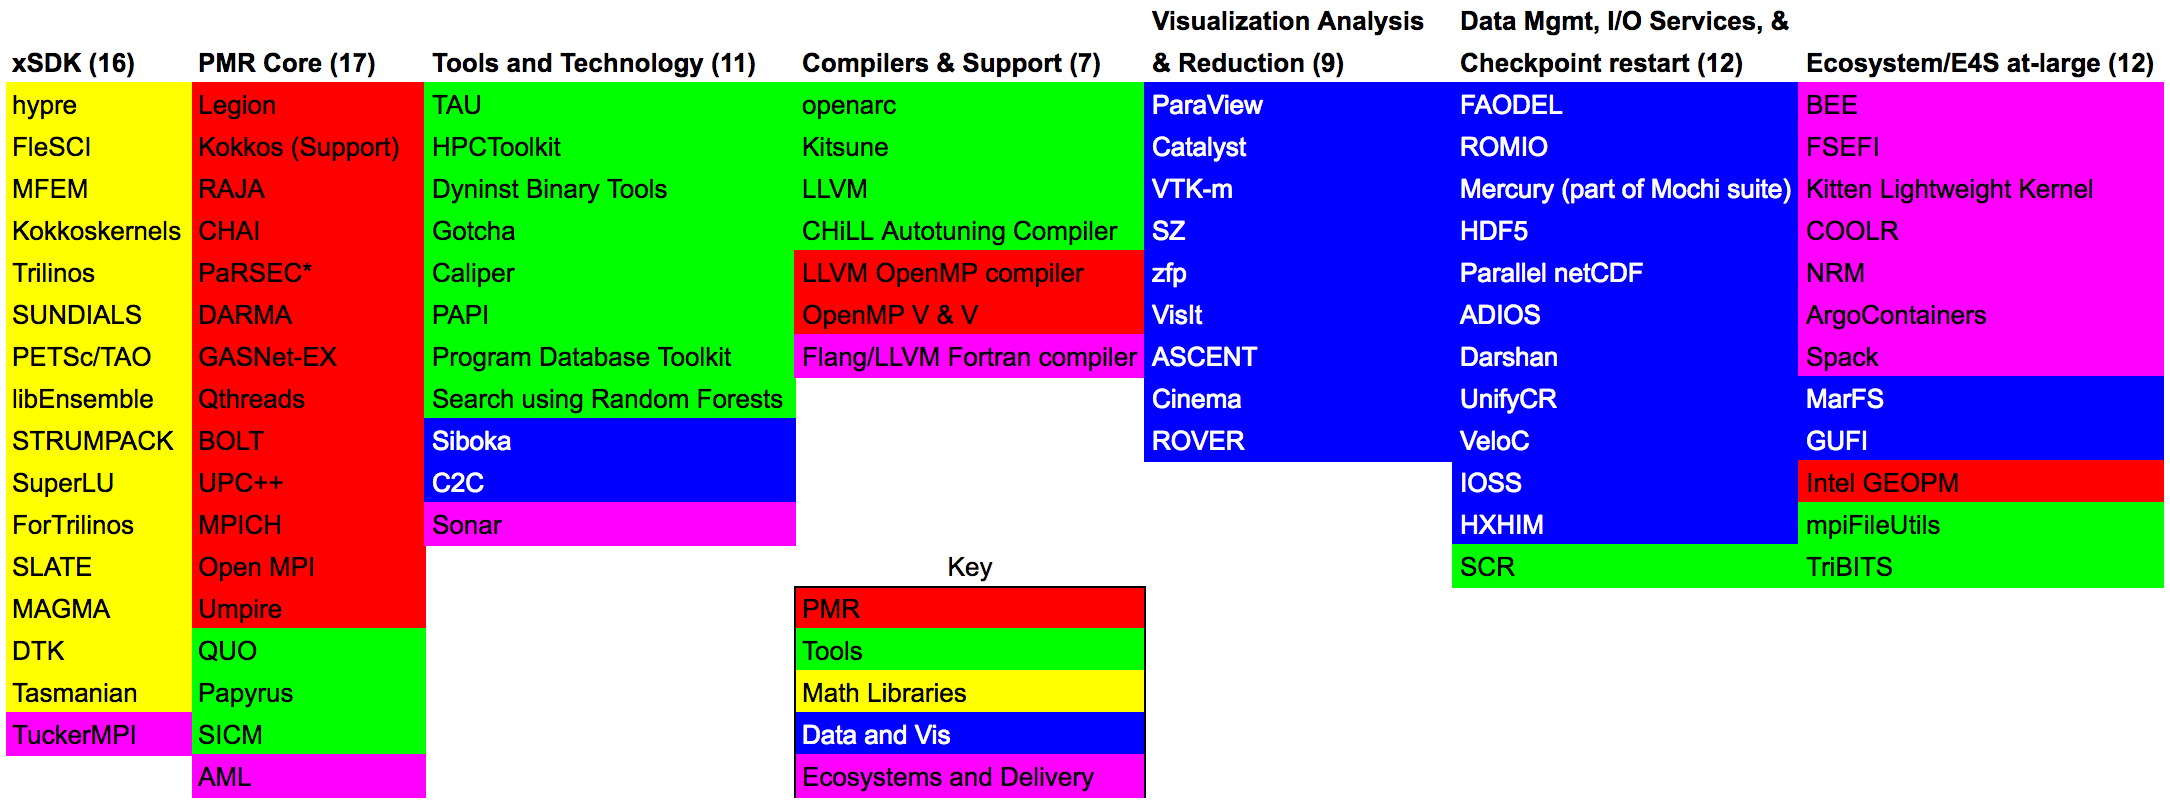
\includegraphics[width=6.5in]{projects/2.3.5-Ecosystem/2.3.5.01-Ecosystem-SDK/SDKdefinition1}
        \caption{\label{fig:sdk-definition1}The above graphic shows the breakdown of ECP ST products into 6 SDKs ( the first six columns).  The rightmost column lists products that are not part of an SDK, but are part of Ecosystem group that will also be delivered as part of E4S. The colors denoted in the key map all of the ST products to the ST technical area they are part of.  For example, the xSDK consists of products that are in the Math Libraries Technical area, plus TuckerMPI which is in the Ecosystem and Delivery technical area.}
\end{figure}

\paragraph{Next Steps}
Current and near-term efforts include:

\begin{itemize}
\item  Defining community policies for E4S.
\item  Assisting with E4S deployment to computing facilities.
\item  Adding additional ST software to E4S for inclusion in the version 1.0 release.
\item  Creating a Spack build-cache for improving the ease of installation of E4S packages. 
\item  Creating a set of reproducible container recipes for E4S SDKs.
\item  Creating base images for Linux x86\_64, ppc64le, and aarch64 architectures.
\item  Beginning SDK-specific community policy discussions within newly formed SDK communities.
\item  Testing new ECP-funded continuous integration capability.
\end{itemize}

